%% LyX 2.3.5-1 created this file.  For more info, see http://www.lyx.org/.
%% Do not edit unless you really know what you are doing.
\documentclass{article}
\usepackage[latin9]{inputenc}
\usepackage{geometry}
\geometry{verbose,tmargin=1in,bmargin=1in,lmargin=1in,rmargin=1in}
\usepackage{float}
\usepackage{fancybox}
\usepackage{calc}
\usepackage{pdfpages}
\usepackage{amsmath}
\usepackage{amsthm}
\usepackage{graphicx}
\usepackage{wrapfig}
\usepackage{setspace}
\usepackage[euler]{textgreek}
\usepackage[authoryear]{natbib}
% \onehalfspacing
\singlespacing
\usepackage[unicode=true,pdfusetitle,
 bookmarks=true,bookmarksnumbered=false,bookmarksopen=false,
 breaklinks=false,pdfborder={0 0 1},backref=false,colorlinks=false]
 {hyperref}
 
\usepackage{supertabular,array,threeparttable}

\makeatletter

%%%%%%%%%%%%%%%%%%%%%%%%%%%%%% LyX specific LaTeX commands.
%% A simple dot to overcome graphicx limitations
\newcommand{\lyxdot}{.}


%%%%%%%%%%%%%%%%%%%%%%%%%%%%%% Textclass specific LaTeX commands.
\theoremstyle{plain}
\newtheorem*{lem*}{\protect\lemmaname}
\theoremstyle{definition}
 \newtheorem{example}{Example}
\theoremstyle{plain}
\newtheorem{prop}{Proposition}
\theoremstyle{plain}
\newtheorem{cor}{Corollary}
\theoremstyle{plain}
\newtheorem*{assumption*}{Assumption}
\theoremstyle{plain}
\newtheorem{assumption}{Assumption}

%%%%%%%%%%%%%%%%%%%%%%%%%%%%%% User specified LaTeX commands.
\usepackage{amssymb}
\usepackage{amsfonts}
%\usepackage[cal=boondoxo]{mathalfa}
\usepackage{hyperref}
\hypersetup{
    colorlinks,
    linkcolor={red!50!black},
    citecolor={blue!50!black},
    urlcolor={blue!80!black}
}

\usepackage{afterpage}

\makeatother

\begin{document}
\title{\vspace{-0.2cm}
Sex differences in COVID-19 mortality in the United States : \newline A state-level analysis\vspace{0.5cm}
}
\author{\normalsize{}Simona Bignami \footnote{Department of Demography, Universit\'{e} de Montr\'{e}al} ,
{\normalsize{}Timothy Riffe\footnote{University of the Basque Country, Ikerbasque and Max Plank Institute for
Demographic Research}} ,
\normalsize{}Daniela Ghio\footnote{Joint Research Centre European Commission} ,
\normalsize{}Pietro Violo\textsuperscript{*},
{\normalsize{}Enrique Acosta}\footnote{Max Plank Institute for Demographic Research} }
\date{\vspace{1.5cm}
EXTENDED ABSTRACT\\ \vspace{1.5cm}
September 2021\\ \vspace{1cm}
Proposed for presentation at the\\Annual Meeting of the
Population Association of America\\
Atlanta, Georgia, April 6-9, 2022\\
}

\maketitle
\vspace{0cm}

\newpage{}
\section*{Abstract}
Male mortality due to COVID-19 has been found to be higher than women's due to a combination of biological and behavioural factors. The United States has been one of the countries most affected by the COVID-19 pandemic, with large variations at the state and county levels in infection and mortality rates. In this paper, we assess sex differentials in COVID-19 mortality across US states and compare them with sex differentials in all-cause mortality, as well as six leading causes of death. We establish the male disadvantage in COVID-19 mortality, which is systematically higher than for all-cause mortality. We also describe the trajectory of male-to-female COVID-19 mortality ratios across ages, showing that male disadvantage decreases significantly in the 85+ age group. Although there is some convergence between states as age increases, Western states consistently exhibit the largest male excess mortality, and Southern States, the lowest.  \\ \\

\noindent \newpage{}

\baselineskip1.5\baselineskip

\section*{Introduction\label{sec:Introduction}}
Since early in the pandemic of the new coronavirus disease (COVID-19), it has been observed that, like for other infectious diseases, COVID-19 case fatality is higher for men than for women \citep{10.1371/journal.pone.0250523}. Overall, male mortality due to COVID-19 is also higher than women's, and the magnitude of sex differences in COVID-19 mortality is larger than for other causes of deaths, especially at older ages \citep{Geldsetzer2021.02.23.21252314,Guilmoto2020.05.17.20097410}, due to a combination of biological and behavioral factors \citep{falahi_sex_2021,cite-key, 10.1371/journal.ppat.1008570,cite-key2,cite-key3}.
The United States has been one of the countries most affected by the COVID-19 pandemic, but with large variation at the state and county levels in infection and mortality rates. Excess mortality, a key demographic indicator used to assess the burden of the pandemic, has been found to be higher among counties with lower median household incomes and less formal education, counties with poorer health and more diabetes, and counties in the South and West\citep{10.1371/journal.pmed.1003571}. Bearing that in mind, we examine state and region-level differentials in COVID-19 mortality and how they compare with all-cause mortality, and look at the trajectory of male excess mortality across ages. This is important to understand to what extent the COVID-19 pandemic will worsen existing sex differentials in mortality in the United States.


\section*{Data and methods}

The mortality data for various diseases, including COVID-19, were extracted from the Centers of Disease Control and Prevention (CDC) website. CDC publishes weekly deaths in which COVID-19 has played a contributing factor, divided by sex, age group and state. We have aggregated the weekly data to obtain the cumulative deaths up until April 15 2021, which corresponds to the beginning of widespread availability of COVID-19 vaccines in the United States. We have decided to not use the most recent data under the assumption that those who died from the disease before and after vaccines were made available to parts of the population have different characteristics. The COVID-19 mortality rates for every state, sex and age group were obtained by dividing the cumulative deaths by the 2019 population (Census Bureau).

Following the approach of \citet{Geldsetzer2021.02.23.21252314}, we calculate male-to-female COVID-19 mortality ratios for each US state. In order to explore how the gender differential in COVID-19 mortality compared with all-cause mortality prior to the emergence of the virus, we extracted mortality rates by state, sex and year of age for the year 2018 from the United States Mortality Database (USMBD). We computed a weighted average of these rates within the age groups available for COVID-19 mortality. For example,
$$ {}_nM_x^{All-cause} = \frac{\sum_{i=x}^{x+n} M_i^{All-cause}\times P_{i}}{\sum_{i=x}^{x+n}P_{i}}$$

In order to conduct comparisons across states, we also produced standardized death rates for COVID-19 and all-cause mortality, using the total population of the United States as the standard population:
$$ SDR = \frac{\sum_i M_i\times P^{US}_{i}}{\sum_iP^{US}_{i}}$$

Our first quantity of interest is the male-to-female mortality ratio for both COVID-19 and all-cause mortality, given by:
$$\frac{SDR_M}{SDR_F}$$

Confidence intervals were built using a Monte Carlo simulation method. We assumed that deaths were Poisson distributed and generated a sample of 1000 male-to-female mortality ratios, which allowed us to identify 95\% confidence intervals.

We then computed the mortality rates of males and females prior to the emergence of COVID-19 for six leading causes of death in order to evaluate how they compare to the novel virus. The causes of deaths selected were Diabetes mellitus, malignant neoplasms, diseases of the circulatory system, diseases of the nervous system, influenza and pneumonia, and other diseases of the respiratory system. The CDC WONDER database was used to request the data of interest, consisting of death counts and rates of each group of diseases, filtered by state, sex and age group, for 2019. 

\\
\section*{Preliminary results}

Age-adjusted COVID-19 and all-cause mortality sex ratios for all states are presented in Figure 1. Confirming the results of earlier studies \citep{Geldsetzer2021.02.23.21252314,Guilmoto2020.05.17.20097410}, we find that COVID-19 mortality is highly gendered. In about half of the states, the age-adjusted male-to-female COVID-19 mortality ratio is significantly higher than the male-to-female all-cause mortality ratio, and in no state is it significantly lower. In addition, gender differentials in COVID-19 mortality increase as the overall level of COVID-19 mortality increases, the difference being highest in the Western states and lowest in the Southern states. Further analyses will attempt to clarify the regional and state differences in male excess mortality from COVID-19. 

In most states, the relative sex differences for COVID-19 were larger than for other common causes of death, but only between age 40 and 60. However, the gender gap in COVID-19's mortality diminishes as we advance in age. This phenomenon is shared with diabetes mellitus, diseases of the circulatory system and of the nervous system. Conversely, we observe the opposite trend in diseases of the respiratory system as well as malignant neoplasms (Figure 3). This striking difference between the trajectories of male-to-female mortality ratios of COVID-19 (Figure 2) and influenza and pneumonia as well as other respiratory diseases is an interesting one: whereas COVID-19 is also a respiratory infection, it exhibits markedly different gender patterns. Notably, the residential situation of American elders might have been a major factor in this result, given the high contagiousness of COVID-19 compared to common contagious respiratory diseases. Although women outnumber men in older ages, they are also more likely to live in collective dwellings. In 2016, 67.5\% of residents in long-term care facilities in the United States aged 80+ were women, and women aged 80+ were 1.7 times more likely to live in long-term care facilities than men aged 80+ (calculations from OECD data, 2021). It can be thought that this gendered difference in living situation and the outbreaks of COVID-19 in collective dwellings led to the attenuation of male excess mortality of COVID-19 in the 85+ age group.

\begin{figure}[h!]
\centering
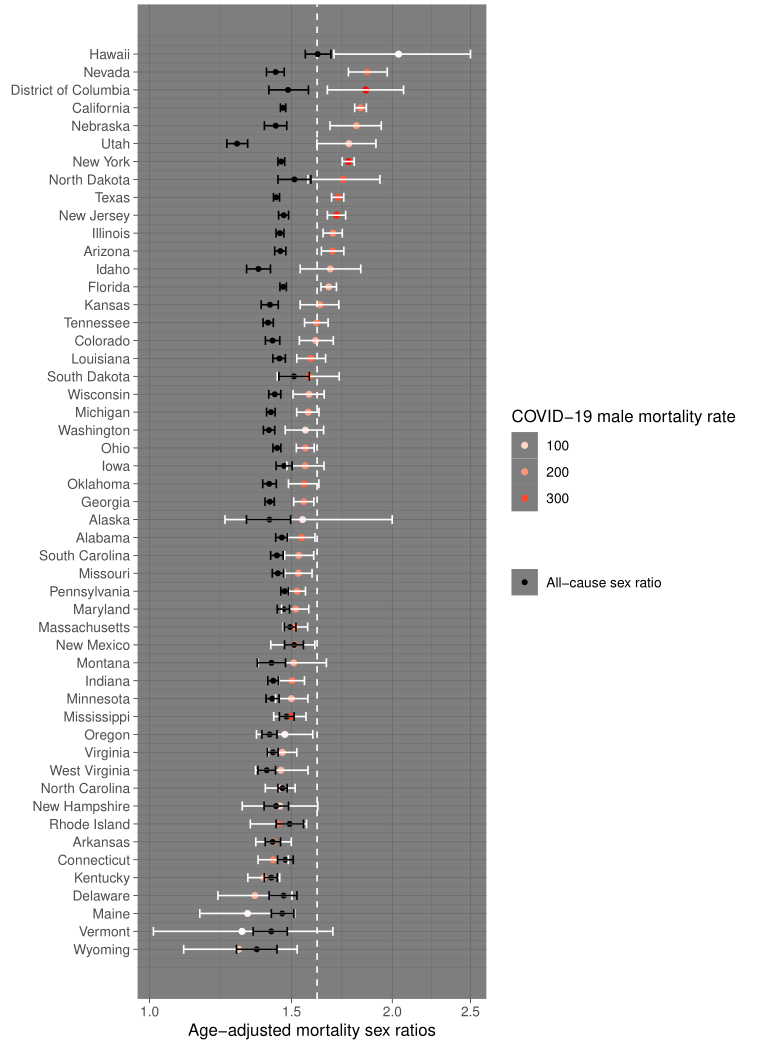
\includegraphics[width=135mm]{Mort.png}
\caption{\textbf{Age-adjusted COVID-19 and all-cause mortality sex ratios for 50 states and the District of Columbia} \newline Source: Author's calculations based on data obtained from weekly CDC publications.}
\label{fig:fig1}
\end{figure}

\begin{figure}[h!]
\centering
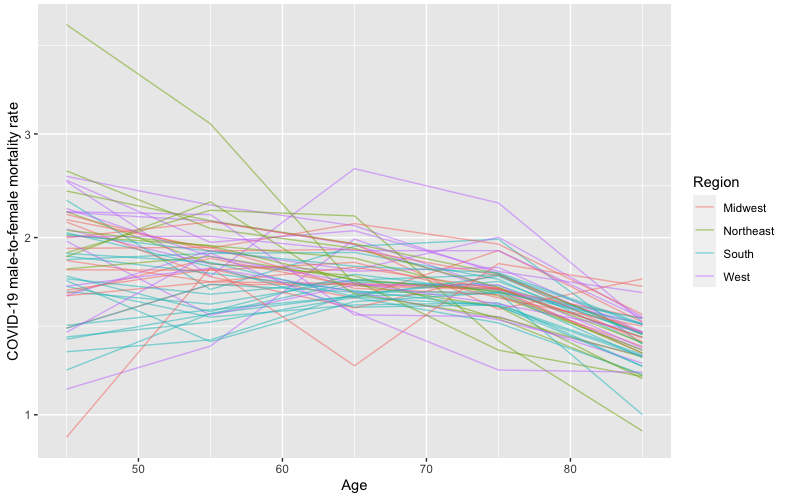
\includegraphics[width=150mm]{Rplot.png}
\caption{\textbf{COVID-19 male-to-female mortality rate across age groups for US States, grouped by US region} \newline Source: Author's calculations based on data obtained from weekly CDC publications.}
\label{fig:fig2}
\end{figure}

\begin{figure}[h!]
\centering
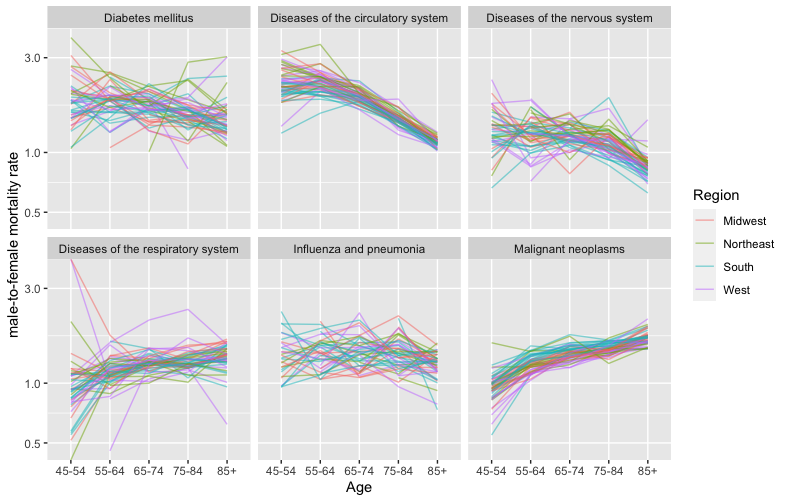
\includegraphics[width=150mm]{Rplot01.png}
\caption{\textbf{Male-to-female mortality rate for six causes of death across age groups, grouped by US region} \newline Source: Author's calculations based on data obtained through CDC WONDER.}
\label{fig:fig3}
\end{figure}


\clearpage
% Bibliography
\nocite{HMD}
\bibliographystyle{chicago}
\bibliography{ref}

\noindent US Census Bureau. "State Population by Characteristics: 2010-2019." \textit{The United States Census Bureau}, https://www.census.gov/data/tables/time-series/demo/popest/2010s-state-detail.html. Accessed 15 April 2021.

\noindent COVID-19 Case Surveillance Public Use Data with Geography | Data. \textit{Centers for Disease Control and Prevention}. https://data.cdc.gov/Case-Surveillance/COVID-19-Case-Surveillance-Public-Use-Data-with-Ge/n8mc-b4w4. Accessed 15 April 2021.

\noindent \textit{United States Mortality DataBase}. University of California, Berkeley (USA). Available at usa.mortality.org (data downloaded on [April 15 2021]).

\noindent \textit{Underlying Cause of Death, 1999-2019 Request}. https://wonder.cdc.gov/ucd-icd10.html. Accessed 15 April 2021.



\begin{table}[ht]
\centering
\caption{Confidence intervals of bootstrapped excess male mortality between COVID-19 and various diseases} 
\begin{tabular}{llrrrl}
  \hline
Age Group & Cause of death & Mean & Lower CI & Upper CI & Is 1 in the CI? \\ 
  \hline
55-64 & Diabetes mellitus & 0.94 & 0.88 & 1.00 & TRUE \\ 
  65-74 & Diabetes mellitus & 0.98 & 0.92 & 1.04 & TRUE \\ 
  75-84 & Diabetes mellitus & 1.07 & 1.00 & 1.16 & TRUE \\ 
  85+ & Diabetes mellitus & 0.99 & 0.91 & 1.06 & TRUE \\ 
  85+ & Diseases of the respiratory system & 1.04 & 0.99 & 1.09 & TRUE \\ 
   \hline
\end{tabular}
\end{table}



\begin{table}[ht]
\centering
\caption{Evolution of COVID-19 male-to-female mortality, United States, 2020-2022} 
\begin{tabular}{lrrr}
  \hline
Age Group & Before& After & After \\ 
  \hline
45-54 & 2.00 & 1.85 & 1.72 \\ 
  55-64 & 1.86 & 1.73 & 1.60 \\ 
  65-74 & 1.78 & 1.68 & 1.55 \\ 
  75-84 & 1.65 & 1.64 & 1.65 \\ 
  85+ & 1.32 & 1.39 & 1.61 \\ 
   \hline
\end{tabular}
\end{table}

\pagebreak 

$$MFR_i = \frac{\frac{^m Deaths_i}{^m Population_i}}{\frac{^f Deaths_i}{^f Population_i}}$$

$$ \text{RMFR} = \frac{MFR_{\text{ COVID-19}}}{MFR_{\text{ Other disease}}}$$

\end{document}



